\documentclass[a4paper,10pt]{article}
\usepackage[utf8]{inputenc}
\usepackage{amsfonts}
\usepackage{tikz}
\usepackage{amsmath}
\usetikzlibrary{arrows}

\title{Telling a Story}
\author{Zongzhe Yuan}

\begin{document}

\maketitle

\section{Initial Approach to the Reduction Problem}
\subsection{Troubles in the Path Problem Solving}
The discussion of the reduction problem originated from an extension of a problem that was not discussed in detail on the L11 Algebra Path Problem class. \\
In that course, we were using the algebraic approaches to represent and calculate the path problem. A path problem will be represented as a semiring and the real case to the problem will be represented and calculated by a matrix semiring constructed from the previous semiring.\\
However, not all real-world problems can be solved directly with the simple matrix semiring. 
For example, we may meet the following situation (node 3 is not connected to all other nodes).\\\\
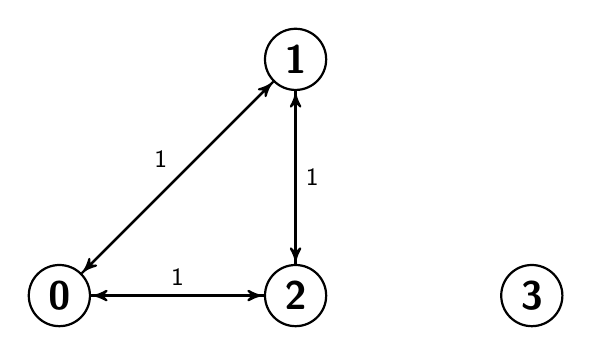
\begin{tikzpicture}[->,>=stealth',shorten >=1pt,auto,node distance=3cm,
                    thick,main node/.style={circle,draw,font=\sffamily\Large\bfseries}]

  \node[main node] (0) {0};
  \node[main node] (2) [right of=0] {2};
  \node[main node] (1) [above of=2] {1};
  \node[main node] (3) [right of=2] {3};

\path[every node/.style={font=\sffamily\small}]
    (0) edge node {1} (2)
        edge node {1} (1)
	(1) edge node {} (0)
        edge node {1} (2)
    (2) edge node {} (0)
        edge node {} (1)
;
\end{tikzpicture}\\\\
We will get the following initial path problem matrix by using the RIP protocol (here need the reference for RIP).
\[
\begin{bmatrix}
    0 & 1 & 1 & \infty \\
    1 & 0 & 1 & \infty \\
    1 & 1 & 0 & \infty \\
    \infty & \infty & \infty & 0 \\
\end{bmatrix}
\]\\
After using the RIP protocol for n-step matrix calculations (multiplication), we obtained such a matrix:
\[
\begin{bmatrix}
    0 & 1 & 1 & n+1 \\
    1 & 0 & 1 & n+1 \\
    1 & 1 & 0 & n+1 \\
    \infty & \infty & \infty & 0 \\
\end{bmatrix}
\]\\
The result shows that if we do not limit the number of steps in the calculation, eventhough we may get the results of the path we need in the early step (eg path from $a$ to $b$), but a better solution for the entire matrix may be found after "many: steps (or the calculation will counting to infinity, which is shown in this example).\\
\section{Possible Solution}
Therefore, in the course L11, instead of using RIP and simple matrix semiring approach, we used another protocol called BGP (here need the reference for BGP). We start from the simple $(\mathbb{N},min,+)$ semiring that calculate the shortest distance, and we use lexicographic product (need reference to the Background/Definition) to construct a new semiring that contains the shortest-path metric and the set of its path.\\\\
(these definition could be moved into definition section)\\
Here we need to define some new operators/new rules for our semigroup:\\
Assume $(S,\bullet)$ is a semigroup. Let $lift(S,\bullet)\equiv (fin(2^S),\hat\bullet)$ where
$X \hat\bullet Y = \{x\bullet y |x\in X,y\in Y\}$.\\
Then we can use our $lift$ to construct a bi-semigroup:\\
Assume $(S,\bullet)$ is a semigroup. Let $union\_lift(S,\bullet)\equiv (\mathcal{P}(S),\cup,\hat\bullet)$ where
$X \hat\bullet Y = \{x\bullet y |x\in X,y\in Y\}$, and $X,Y \in \mathcal{P}(S)$, which is the set of finite subsets of $S$.\\
Then for a given graph $G = (V,E)$, we define $path(E)\equiv union\_lift(E^*,.)$ where . is the concatenation function of sequence.\\
Finally we get our "shortest paths with paths" semiring from a given graph $G = (V,E)$: $spwp \equiv AddZero(\bar0,(\mathbb{N},min,+) \overrightarrow{\times} path(E))$.\\
\subsection{Introduce Reduction into Our Problem}
Here comes to the problem, when we are using $spwp$ for doing calculations, because there may have loops in our $path(E)$, we need a lot of extra computation (though it will eventually yield correct results) to prove the paths have loops are not the shortest path.
In order to eliminate these paths with loops, we introduced a new concept in the L11 course, the reduction.\\\\
If $(S,\oplus,\otimes)$ is a semiring and $r$ is a function from $S$ to $S$, then $r$ is a reduction if $\forall a,b \in S$, $r(a) = r(r(a))$, $r(a\oplus b) = r(r(a)\oplus b) = r(a\oplus r(b))$ and 
$r(a\otimes b) = r(r(a)\otimes b) = r(a\otimes r(b))$.\\
And, if $(S,\oplus,\otimes)$ is a semiring and $r$ is a reduction, then $red_r(S) = (S_r,\oplus_r,\otimes_r)$, where $S_r = \{s\in S|r(s)= s\}$, $x\oplus_r y = r(x\oplus y)$ and $x\otimes_r y = r(x\otimes y)$.\\
After that we went back to our path problem that for a given path $p$, we say $p$ is elementary if there is no node inside $p$ that is repeated. Then we can define our elementary path using the reduction $r(X) = \{p\in X | p $ is elementary$\} $ and $epaths(E) = red_r(paths(E))$.\\\\
Therefore, our path problem semiring became to $AddZero(\bar0,(\mathbb{N},min,+) \overrightarrow{\times} epath(E))$.\\\\
However, we still encounter the problem that there exists elements in our problem set that has a path distance value but does not have edges in its path. So we need to define the second reduction, which turns all elements that don't satisfy the condition into a single element (the $zero$ we added into our semiring).\\
$r_2 (inr(\infty)) = inr(\infty)$, $r_2 (inl(s,\{\})) = inr(\infty)$ and $r_2 (inl(s,W)) = inl(s,W)$ where $W$ is not empty.
Therefore, our path problem semiring becomes to $red_{r_2}(AddZero(\bar0,(\mathbb{N},min,+) \overrightarrow{\times} epath(E)))$.\\\\
It is worth mentioning that we did not discuss the properties of reduction in detail in the L11 course. We also did not know whether the original semiring still satisfies the semiring property after the reduction. At the same time, whether some properties of the original operators (such as commutative rules) remains or not after reduction is also a mystery to us.\\
These are the topics that we need to focus on in our discussion.
It is worth mentioning that the first reduction (reduce all pathes that are not elementary) that we defined above does not follow the property of the reduction on the $min$ operation (doesn't have left/right invariant property). Imagine we have path $A = \{a,b,c,d\}$ that is longer but does not have loop and $B = \{a,b,b\}$ that is shorter but does have loop. Then $r(A\oplus B) = r(B) = \infty$ because $B$ is shorter but has loop, but $r(A\oplus r(B)) = r(A \oplus \infty) = r(A) = A$ because $B$ has loops but $A$ doesn't.\\
Therefore, we not only discuss the properties of reduction, but also try to find another way to represent reduction to solve our path problem.
\section{Classical Reduction and Example}
In order to better understand reduction and further analyze it in detail, we trace the source to find out if there is any other definition and study of reduction before us. 
In fact, the earliest definition we could find about reduction came from Ahnont Wongseelashote in 1977\cite{WONGSEELASHOTE197955}. Wongseelashote also encountered the problem similar to ours when studying the path problem in the paper. In fact, our definition of reduction is very similar to Wongseelashote's definition of reduction (the real reason is that L11 refers to the Wongseelashote definition when the definition of reduction was given). However, unfortunately, Wongseelashoth only put forward the concept of reduction in the paper without detailed reasoning and structure proof.\\
Next we found that Alexander James Telford Gurney also mentioned the concept of reduction in his Ph.D thesis\cite{gurney_construction_2010}. Gurney's discussion of reduction is also based on the definition by Wongseelashote, and it also does not focus on reduction for detailed structure proof.\\\\
Therefore, we can temporarily use the previously mentioned definition of reduction as “classical reduction” and do reasoning on it at first (because it does not satisfy our elementary path problem and is extraction and implementation un-friendly, so we call it classical).\\
To help us understand reduction and study its properties, we found another example of reduction in the course of L11.\\\\
The reduction is call $min_{\leq}$ (Martelli’s semiring)\cite{martelli_gaussian_1976} which means removing all the superset.
For a given graph $G = (V,E)$, A cut set $C \in E$ for nodes $i$ and $j$ is a set of edges such there is no path from $i$ to $j$ in the graph $(V, E - C)$. $C$ is minimal if no proper subset of $C$ is a cut set. And Martelli’s semiring is such that $A^{(*)}(i, j)$ is the set of all minimal cut sets for $i$ and $j$. 
So Martelli’s semiring =$(S,\oplus,\otimes,\bar0,\bar1)$ where $S = min_\leq(2^{2^E})$, $X\oplus Y = min_\leq(\{U \cup V | U \in X, V \in Y\})$, $X\otimes Y = min_\leq(X \cup Y)$, $\bar0 = \{\{\}\}$ and $\bar1 = \{\}$.\\
Here we can easily prove that $min_\leq$ satisfies our previous definition of reduction. So $min_\leq$ is a classical reduction. (I am considering whether or not paste the proof of matrelli's semiring)
\section{Generalized Reduction}
\subsection{Traditional Representation}
The previous section have mentioned that our definition of classical reduction is implement un-friendly.
This is because inside classical reduction our actual problem set is $S_r = \{s\in S|r(s)= s\}$ which is a type with record. Record is difficult to be accurately represented in most situations. 
Imagine we have two different reductions $r_1$ and $r_2$ for $S$, then the problem set after applying reduction $r_1$ and $r_2$ will be $S_r = \{y\in \{x \in S | r_1(x) = x\}|r_2(y)= y\}$. 
The nest record of reduction in our problem domain makes all the reasoning and calculation step into trouble. 
At the same time, since our real problem set has changed from the original $S$ to the current $S_r = \{s\in S|r(s)= s\}$ (suppose we only have one reduction $r$), the domain of our operator/relationship have changed. If we originally have a binary operator $\oplus : S \rightarrow S$, then the binary operator after reduction will become the binary operator $\oplus_r : \{s\in S|r(s)= s\} \rightarrow \{s\in S|r(s)= s\}$. And if we apply two/more reductions simultaneously, the entangling of reductions with problem set and relationship/operator makes it almost impossible for us to define the combinator that exists on reduction and solve the problem at all. 
Taking into account the elementary path problem we previously focused on, the reduction does not satisfy the properties of classical reduction, so we need to represent/generalize our reduction in a new way.\\
\subsection{Generalized Reduction Representation}
How to generalize reduction is exactly what we need to consider.
First we take the binary relationship, the equality, as the starting point.\\
If there is an equality $=$, which is a binary relationship, on the original problem set $S$, then it is obvious that the equality $=_r$ on the reduced problem set  $S_r = \{s\in S|r(s)= s\}$ will no longer to be $=$ any more. If we have $x,y \in \{s\in S|r(s)= s\}$, because we have $r(x) =x$ and $r(y) = y$, then $x =_r y \leftrightarrow r(x) = r(y)$. So we can represent the equality on the reduced set as $\forall x,y \in \{s\in S|r(s)= s\}, x =_r y \equiv r(x) = r(y)$.\\
For the same problem, we need to generalize the binary operator under the reduction type as well.
If we originally have a binary operator $\oplus : S \rightarrow S$, then the binary operator after reduction will become the binary operator $\oplus_r : \{s\in S|r(s)= s\} \rightarrow \{s\in S|r(s)= s\}$. Considering that $r(x) =x$ and $r(y) = y$, the binary operator $\oplus_r$ could be represent as $\forall x,y \in \{s\in S|r(s)= s\}, x \oplus_r y \equiv r(r(x) \oplus r(y))$.\\
\subsection{Generalised Reduction and Its Properties}
\subsubsection{General Properties}
After having a new representation method, we need to prove the equivalent of this new method and the classical reduction on representation.\\
Here we mainly focus on the equivalence of these properties:\\
Reflexive, Symmetric, Transitive and Congruence for equality(binary relationship) and\\
Commutative, Associative, Selective, Congruence, Has Identity and Has Annihilator for the binary operator.\\
First of all, we use the classical reduction representation to represent these properties.\\
If we have a semigroup $(S,\oplus)_=$, then the reduced semigroup will be $(S_r,\oplus_r)_{=_r}$, where\\
$S_r \equiv \{s\in S|r(s)= s\}$, \\ 
$\forall a,b \in \{s\in S|r(s)= s\}, a =_r b \equiv \pi_1a = \pi_1 b$ ($\pi$ is the projection function, since the reduced set is represented as a record, we can project the first/second element from the record),and\\
$\forall a,b \in \{s\in S|r(s)= s\}, a \oplus_r b \equiv (r(\pi_1x \oplus \pi_1y), r(r(\pi_1x \oplus \pi_1y)) = r(\pi_1x \oplus \pi_1y)) \in \{s\in S|r(s)= s\}$.\\
In this representation, we can clearly see that the original representation of classical reduction is very implement unfriendly.\\
Next we try to represent the same problem with our newly defined representation method.\\
If we have a semigroup $(S,\oplus)_=$, the reduced semigroup will be $(S,\oplus_r)_{=_r}$, where\\
$\forall a,b \in S, a =_r b \equiv r(a) = r(b)$, and\\
$\forall a,b \in S, a \oplus_r b \equiv  r(r (a) \oplus r(b))$.\\
Finally, we need to show that the properties in the classical representation is isomorphic to the properties in our new representation.\\
$\forall a \in \{s\in S|r(s)= s\}, a =_r a \equiv \pi_1a = \pi_1 a \longleftrightarrow \forall a \in S, a =_r a \equiv r(a) = r(a)$ (reflexive)\\
and more examples, includes equality and binary operator\\\\
It is worth mentioning that in our new form of representation, if reduction has a left/right invariant property on the binary operator, then we can conclude that $\forall a,b \in S, a \oplus_r b \equiv  r(r (a) \oplus r(b)) = r (a \oplus b)$. 
But on the other hand, it also shows that our new reduction representation can be used to represent a reduction that does not have an left/right invariant property (such as the reduction we mentioned earlier in the elementary path problem which does not have those properties on $min$ operator).
This also solves the problem we previously mentioned that classical reduction cannot be used to define the reduction that we need.\\
\subsubsection{Associative and Pseudo-Associative}
Among all the properties of binary operators 
(commutative, associative, selective, congruence, has identity and has annihilator), the associative law is the most special one. 
Taking the proof of commutative law as an example:\\
$\forall a,b \in S, a \oplus_r b \equiv  r(r (a) \oplus r(b)) =_r r(r (b) \oplus r(a)) \equiv b \oplus_r a$. And by the definition of $=_r$ we get $r(r (a) \oplus r(b)) =_r r(r (b) \oplus r(a)) \equiv r(r(r (a) \oplus r(b))) = r(r(r (b) \oplus r(a)))$. 
It is obvious that in the proof, we only need to use the commutative law of the original binary operator, which is $\forall a,b \in S, a \oplus b = b \oplus a$, and the property of the congruence of our reduction, which is $\forall a,b \in S, a = b \rightarrow r(a) = r(b)$. However, the proof of associativity is not the same. The proof of associative will become $\forall a,b,c \in S, (a \oplus_r b) \oplus_r c  \equiv  r(r(r (a) \oplus r(b)) \oplus r(c)) =_r r(r (a) \oplus r(r(b) \oplus r(c))) \equiv a\oplus_r (b \oplus_r c)$. In the proof we not only need the associative law of the original binary operator, which is $\forall a,b,c \in S, (a\oplus b) \oplus c = a \oplus (b\oplus c)$, and the property of the congruence of reduction, but also need our reduction to have the property of left/right invariant.\\
We've mentioned earlier that the reduction we expect in the elementary path problem does not have these properties on the $min$ operator. However, we hope to prove its associative property on both operator in the elementary path problem. So we hope to have a better way to represent associative under reduction, and we call it pseudo-associative: $\forall a,b,c \in S, r(r(r(a)\oplus r(b)) \oplus r(c)) = r(r(a) \oplus r(r(b)\oplus r(c)))$. And we can prove that pseudo-associative and associative under reduction are isomorphic, which means the left/right invariant is only a sufficient condition to associative property, but not a sufficient and necessary condition.\\
So our defined generalize reduction solves both the problem of that the traditional representation is implemented unfriendly and the inability to represent reduction without the left/right invariant properties for classical reduction, by finding another way to prove associative for those reductions that don't have left/right invariant properties.\\
\subsubsection{Distributivity}
What we need to discuss next is the issue of the distribution of two operators on semiring, which is left distributive $\forall a,b,c \in S, a\otimes (b \oplus c) = a \otimes b \oplus a \otimes c$ and right distributive $\forall a,b,c \in S, (a \oplus b) \otimes c = a \otimes c \oplus b \otimes c$.
We need to discuss whether or not the original semiring remains the property of distributive law after our reduction. \\
As what we did in the previous section, we should discuss the problem beginning  with  the classical reduction. We are very surprised to find that if our reduction is classical and we have left/right invariant properties on both operators, then our semiring can remain the distribution property after reduction.\\
We also mentioned in the previous section that the traditional representation of reduction is equivalent to the generalize representation we defined in this section, which indicates that the sufficient condition to that the semiring remains the distributive law is the properties of the left/right invariant.\\
$\forall a,b,c \in S,  a \otimes_r (b \oplus_r c)  \\
= r(r(a) \otimes r(r(r(b)\oplus r(c)))) $ by the definition of $\oplus_r$ and $\otimes_r$\\
$= r(r(a) \otimes r(r(b)\oplus r(c))) $ by the right invariant property of $\otimes_r$\\
$= r(r(a) \otimes r(b \oplus c)) $ by the left and right invariant property of $\oplus_r$\\
$= r(r(a) \otimes (b \oplus c)) $ by the right invariant property of $\otimes_r$\\
$= r((r(a) \otimes b) \oplus (r(a) \otimes c)) $ by the distributive law of $\oplus$ and $otimes$\\
$= r((r(a) \otimes r(b)) \oplus (r(a) \otimes r(c))) $ by the right invariant property of $\otimes_r$\\
$= r(r(r(a) \otimes r(b)) \oplus r(r(a) \otimes r(c))) $ by the left and right invariant property of $\oplus_r$\\
Qed.\\\\
Similarly, in the proof of right distributive law, we need left/right invariant properties of $\oplus_r$ and left invariant property of $\otimes_r$.
Considering the same problems as we met in the previous associative proof, we here regard the relationship between distributive law and reduction as a separate property, pseudo-distributive.
Because sometimes our reduction does not satisfy the left/right invariant properties, it still has the opportunity to allow the semiring to preserve the properties of the distributive law by satisfying the pseudo-distributive law. Here we just state that the left/right invariant property is only a sufficient condition for the semiring to retain the properties of the distributive law rather than a necessary and sufficient condition. \\
pseudo-left-distributive: $\forall a,b,c \in S, r(r(a) \otimes r(r(b)\oplus r(c))) = r(r(r(a) \otimes r(b)) \oplus r(r(a) \otimes r(c)))$, and \\
pseudo-right-distributive: $\forall a,b,c \in S, r(r(r(a) \oplus r(b)) \otimes r(c)) = r(r(r(a) \otimes r(c)) \oplus r(r(b) \otimes r(c)))$. \\
In the later section we will discuss further on the reason that our reduction satisfies pseudo-distributive property when it is satisfying certain specific properties.
\section{Predicate Reduction}
In the previous section we discussed the representation of generalize's reduction, its properties, and that it is isomorphic to traditional reduction. In order to better implement the construction of the path problem we mentioned earlier, we define a type of reduction and perform detailed reasoning on its properties in this section. 
If we deeply consider our reduction, whether it is to eliminate the path with a loop, or to turn an unqualified element tuple into a specific element --additive identity/multiplicative annihilator, we can easily find that our reduction is in the situation that a predicate is set to reduce the elements that satisfy/not satisfy the condition. Therefore, we call this kind of reduction as predicate reduction.\\\\
Initially for our problem set $S$, we define a predicate $P$, which is a function from $S$ to $bool$ and we need to provide a specific element $c$ (the predicate reduction will reduce all the element that satisfied the predicate to $c \in S$). Then we can define the predicate reduction as $\forall a \in S,  r_p(a)=\left\{
\begin{aligned}
c &  & P(a) = true \\
a &  & otherwise 
\end{aligned}
\right.$\\
We also mentioned in the previous chapters that the reduction we defined represented by the generalize method does not necessarily have the properties of left/right invariant. 
But as a reduction it must have the properties of the idempontent and congruence, which are $\forall a \in S, r(a) = r(r(a))$ and $\forall a,b\in S, a = b \rightarrow r(a) = r(b)$. So we need to analyse these two properties. For the property of the idempotent, we need to discuss the input element, split the case that the element satisfies the predicate or not. If the element doesn't satisfy the predicate, then $r(a) = a = r(r(a))$. If the element does satisfy the predicate, then $r(a) = c$ and $r(r(a)) = r(c)$, hence we need to prove/provide the property that $c$ must satisfy the predicate $P(c) = true$. For the property of the congruence, we can conclude from $\forall a,b \in S, r_p(a)=\left\{
\begin{aligned}
c &  & P(a) = true \\
a &  & otherwise 
\end{aligned}
\right. = 
r_p(b)=\left\{
\begin{aligned}
c &  & P(b) = true \\
b &  & otherwise 
\end{aligned}
\right.$ that we need a property $\forall a,b \in S, a = b \rightarrow P(a) = P(b)$, which is the congruence of the predicate $P$.\\\\
Next we need to reduce the binary operator according to the generalize reduction we defined earlier. For our problem set $S$ and a given binary operator $\oplus$, we defined reduced binary operator as $\forall a,b \in S, a \oplus_r b = r_p (r_p(a) \oplus r_p(b))$.\\
Since we completely use the generalize reduction representation defined in the previous section, the reduction we defined has all the above-mentioned properties, such as commutative, selective, congruence, and so on. What deserves our attention is the associative law of a single binary operator and the distribution law of reduce semiring.\\
We also mentioned above that under our generalize reduction representation, the reduction we defined may not satisfy the properties of the left/right invariant (like the $min$ operator under the elementary path problem), so we need to prove (or give certain preconditions) that our reduction to satisfy the pseudo-associative and pseudo-distributive law.\\
Here for our predicate reduction, we found several interesting properties, that is the relationship for the predicate on the elements before/after the binary operation.\\
For a problem set $S$, a given binary operator $\oplus$ and a predicate $P$, we have\\
Predicate-Decomposition : $\forall a,b \in S, P(a \oplus b)= true \rightarrow P(a) = true \bigvee P (b) = true$.\\
Predicate-Composition : $\forall a,b \in S, P(a) = true \bigvee P (b) = true \rightarrow P(a \oplus b)= true$.\\ 
From the property of decomposition we can infer that $\forall a,b \in S, P(a) = false \bigwedge P (b) = false \rightarrow P(a \oplus b)= false$, which means the binary operator will not create elements that satisfy the predicate condition from the elements that don't satisfy the condition.\\
From the property of decomposition we can infer that $\forall a,b \in S, P(a \oplus b)= false \rightarrow P(a) = false \bigwedge P (b) = false$, which means the result of the binary operation will decide the predicate condition of its arguments.\\
Generally speaking, because our additive component of the semiring is mostly selective, then most of our additive components have decomposition properties. At the same time, because our multiplicative component is generally the role of an accumulator, it also makes the composition of this property important for multiplicative components.\\
Let us discuss the above two properties at the level of reduction. If a predicate is decomposed/composition on an operator, it means that the reduction formed by this predicate has the following properties on this operator.\\
$\forall a,b \in S, r_p(a\oplus b) = c \rightarrow r_p(a) = c \bigvee r_p (b) = c$, which is 
$\forall a,b \in S, r_p(a) = a \bigwedge r_p (b) = b \rightarrow r_p(a \oplus b)= a \oplus b$, or\\
$\forall a,b \in S, r_p(a) = c \bigvee r_p (b) = c \rightarrow r_p(a \oplus b)= c$, which is 
$\forall a,b \in S, r_p(a\oplus b) = a \oplus b \rightarrow r_p(a) = a \bigwedge r_p (b) = b$.\\
It is clear that these two properties help us determine the relationship between element and operator under reduction.\\
We first discuss the property of composition. 
We have found that reduction and operator with composition are both left/right invariant.
In other words, composition means that reduction is traditional. According to our previous proof, it also means that this operator retains the property of the associative law under reduction.\\
$\forall a,b \in S, r_p(r_p(a) \otimes b)$. Then we do case analysis on $P(a)$ and $P(b)$:\\
$r_p(r_p(a) \otimes b) = r_p(c \otimes b) = c = r_p(a \otimes b)$, by $P(a) = true$, $P(b) = true$, $P(c) = true$, $P(a \otimes b) = true$ (composition property) and $P(c \otimes b) = true$ (composition property).\\
$r_p(r_p(a) \otimes b) = r_p(c \otimes b) = c = r_p(a \otimes b)$, by $P(a) = true$, $P(b) = false$, $P(c) = true$, $P(a \otimes b) = true$ (composition property) and $P(c \otimes b) = true$ (composition property).\\
$r_p(r_p(a) \otimes b) = c = r_p(a \otimes b)$ by $P(a) = false$, $P(b) = true$, composition property, congruence of $\otimes$ and congruence of $r_p$.\\
$r_p(r_p(a) \otimes b) = r_p(a \otimes b)$ by $P(a) = false$, $P(b) = false$, congruence of $\otimes$ and congruence of $r_p$.\\
Thus, we can conclude that $\forall a,b \in S, r_p(r_p(a) \otimes b) = r_p(a \otimes b)$, which is the left invariant property. We can do the same proof for right invariant property.\\
Next we need to discuss the property of decomposition. We find that if the predicate reduce element (c) is the identity/annihilator for the operator, then the operator has pseudo-associative property after reduction, which we have proved that is isomorphic to the associative property under reduction (the proof needs too many case analysis, that we only provide the Coq proof version instead of formal mathematical proof).\\\\
Then comes to the topic of our greatest concern, the law of distributive. Earlier we mentioned that the left/right invariant is a sufficient condition for the reduction remaining distributive property. Here we hope to try to solve the problem of distributive law from the perspective of predicates.\\
$\forall a,b,c \in S, r_p(r_p(a) \otimes r_p(r_p(r_p(b) \oplus r_p(c))))$. \\
First of all, whether any of a, b, c satisfies predicate $P$, then the result is definite, and the distributive property remains after reduction.\\
The most critical problem is that a, b, and c alone does not satisfy predicate $P$, but $a \otimes b$ or $a \otimes c$ does. We assume that $b \oplus c = b$, $P(a \otimes b) = true$ and $P(a \otimes c) = false$. It is obvious that $r_p(r_p(a) \otimes r_p(r_p(r_p(b) \oplus r_p(c)))) = r_p(a \otimes b) = c$, However $r_p(r_p(r_p(a) \otimes r_p(b)) \oplus r_p(r_p(a) \otimes r_p(c))) = a \otimes c$, which means the distributive law doesn't hold after reduction.\\
So we need to try to stop this kind of thing from happening.\\
First we can make $P(a \otimes b)$ be forced to false, if both $P(a)$ and $P(b)$ are false, and this is our decomposition property. However, as we said earlier, most of our multiplicative components are composition rather than decomposition.\\
Then from a different perspective, we can force $P(a\otimes c)$ to false. From our assumption we have $b \oplus c = b$, then we have $(a \otimes b) \oplus (a \otimes c) = (a \otimes b)$ by the congruence of $\oplus$ and $otimes$. 
Since our additive component is selective, we implicitly define a partial order in our problem set $\forall a,b \in S, a \oplus b = a \longleftrightarrow a \leq b$. 
So we think that if our predicate preserve order on the additive component, both $\forall a,b \in S, a \leq b \rightarrow P(a) = true \rightarrow P(b) = true$, then we can achieve our purpose.\\
However, we were also surprised to find that if an operator is selective and preserve order, then the reduction is traditional (has left/right property) on this operator.
So far, although we have found proof that the distribution law is preserved when both operators are decomposing, for the most of the time, the preservation of distributive law still depends on the property of traditional reduction, namely left/right invariant.\\\\

\section{Construct the Path Problem Semiring}
After the general reasoning of predicate reduction, we used predicate reduction to define three concrete reductions. These three reductions will be used in the construction of our final path problem semiring in the later section. \\\\
In the previous introduction we mentioned the two reductions of elementary path and reduce pair annihilator. The third reduction we used in constructing the final semiring is working on $(\mathbb{N},min,+)$. As mentioned earlier, our path problem is represented by a tuple, which is the path problem with path $(d,P)$. The distance in our path is calculated by $(\mathbb{N},min,+)$ semiring. However, sometimes the distance is too long, which means that some problems may occur during the calculation (for example, an infinite loop in calculation). In addition, in practical applications, we will consider limiting the length of the path. Long paths will not be considered by us. So we can define a reduction that will reduce all long paths distance into one element, we call it ceiling, and the reduction semiring problem is called min plus with ceiling problem. $\forall n \in \mathbb{N}, r_c(n) = \left\{
\begin{aligned}
ceiling &  & n \geq ceiling \\
n &  & otherwise 
\end{aligned}
\right.$ and the predicate here is that $\forall n \in \mathbb{N}, n \geq ceiling$.\\
Since we still use predicate reduce to define reduction here, properties such as commutative and selective have already been proved in the previous part using the properties of predicate reduce. 
So we only care about the property of the predicate itself, and the relationship between the predicate and the operator.\\
First taking into account, we can easily obtain these two properties: $P(ceiling) = true$ which is $ceiling \geq ceiling$ and $\forall a,b \in \mathbb{N}, a = b \rightarrow P(a) = P(b)$ which is $a = b \rightarrow a \geq ceiling = b \geq ceiling$. With these two properties, we can infer from our previous proof that the reduction we defined satisfies the properties of the idempotent and congruence.\\
Next we begin to discuss the relationship between the predicate and operators. \\
We find that our defined predicate is decomposition and preserve order on the $min$ operator.
Decomposition: $\forall a,b \in \mathbb{N}, P(min $ $a$ $b) = true \rightarrow P(a) = true \bigvee $(actually is $\bigwedge$) $P(a) = true$, because $\forall a,b \in \mathbb{N}, min $ $a$ $b \geq ceiling \rightarrow a \geq ceiling \wedge b \geq ceiling$.\\
Preserve order: $\forall a,b \in \mathbb{N}, a \leq b$, (which means $min $ $a$ $b = a$), and $P (a) = true \rightarrow P(b) = true$, because $\forall a,b \in \mathbb{N}, b \geq a \wedge a \geq ceiling \rightarrow b \geq ceiling$.\\
We also find that our defined predicate is composition on the $+$ operator.\\
Composition: $\forall a,b \in \mathbb{N}, P(a) = true \bigvee P(b) = true \rightarrow P(a + b) = true$, because $\forall a,b \in \mathbb{N}, a \geq ceiling \vee b \geq ceiling \rightarrow a + b \geq ceiling$.\\
From our previous proof, we can conclude that since the predicate is preserving order on $min$ and it is composition on $+$, the reduction we defined is both traditional on $min$ and $+$, and has both left/right invariant properties. 
This means that inside our reduced semiring, the reduced $min$ and reduced $+$ operator both retain the associative property, and the combination of the two also has the property of the distributive.\\
At this point, we finish the first reduce semiring built by predicate reduction, and this is also the first half part of the problem that we ultimately need to solve.\\\\
The second predicate reduction we need to define is the reduction that reduce all the path that has loop. First of all, we need to consider how to express our path. For a graph $G = (V,E)$, our problem set should be $\mathbb{P}(E^*)$. However, in fact, we can also use $V$ to represent the path, and this representation is more convenient for us to calculate. For a path $p$ that passes through several points $n_1,n_2 ... n_k \in V$ in turn, we use an ordered list to represent the path $p = [n_1,n_2 ... n_k]$. 
Since the node here is just a reference for a name, in order to facilitate our proof and calculation, we define our path $P = List(\mathbb{N})$, using the natural number to indicate nodes.\\
Next we need to define our two binary operators, min and concat. 
Before defining min we need to define a helper binary order: dictionary order $\forall a,b \in Path,\\ d(nil,b) = nil\\
d(a,nil) = nil\\
d(a::as,b::bs) =
\left\{
\begin{aligned}
a &  & a \leq b \\
b &  & otherwise 
\end{aligned}
\right.$.\\
Then we can use the dictionary order to define our $min$ operator as additive component: \\
$\forall a,b \in Path, min(a,b) = \left\{
\begin{aligned}
a &  & length(a) \leq length(b) \\
d(a,b) &  & length(a) = length(b) \\
b &  & otherwise 
\end{aligned}
\right.$\\
Then the $concat$ operator as the multiplicative component is just the simple concat function of list.\\
Finally we should define the predicate: there has loops in the path. It is really easy since if a path has loop, it must pass at least node more than one times. 
Therefore, as long as there is a duplicate in the list represented for a path, it means that there is a loop in this path.\\
$\forall p \in Path, P(p) \equiv dup(p)$.\\
However, the next problem we have is that there is no identity/annihilator for our additive/multiplicative component in our problem set, since there is no path with infinity length.
Analogous to the previous min plus problem, there is no infinite element in it as well. In the previous question, we manually added a ceiling into the reduction and made it an identity/annihilator for our additive/multiplicative component. However, in this issue we cannot do the same thing. 
Hence we need to manually add an identity/annihilator for our additive/multiplicative component using disjoint union, and our problem set becomes $c + list(\mathbb{N})$.\\
So we can define our reduction as $\forall p \in (c + Path), r(inl(c)) = inl(a)\\
r(inr (a))
\left\{
\begin{aligned}
inl(c) &  & P(a) = true \\
inr(a) &  & otherwise 
\end{aligned}
\right.$.\\
In the same way, we can simply prove two properties $P(inl c) = true$ and $\forall a,b \in (c + Path), a = b \rightarrow P(a) = P(b)$. So we can simply prove the properties of the reduction that we defined here for congruence and idempotent.\\
Next we also need to discuss the relationship between predicates and binary operators. 
We can prove that the predicate is decomposition on $min$ and composition on $concat$. \\
Because our definition of the $min$ operator is selective, it is obvious that it is decomposition on the predicate. \\
For $concat$ operator, it is very similar to the previous $+$ on $\mathbb{N}$ that there is a loop in any of the arguments to the operator will lead to the result of $concat$ yields a loop path. At the same time, we can conclude the traditional property: left/right invariant for the reduction on the $concat$ operator by our previous proof. 
Further we can also prove the associativity property for the $concat$ operator. 
However, it is worth noting that the $concat$ operator does not have the commutative property and it is easy to find the example, because the $list$ is ordered list, $[1] ++ [2] \neq [2] ++ [1]$.\\
The trouble is that our $min$ operator does not preserve order under predicate. 
We can easily find counterexamples: $p_1,p_2 \in Path, length (p_1) < length(p_2) \rightarrow min(p_1,p_2) = p_1, dup(p_1) = true, dup(p_2) = false, P(inr(p_1)) = true, P(inr(p_2)) = false$. 
This means that our reduction is not traditional on $min$ and does not have the property of left/right invariant.\\
Fortunately we can still prove that the $min$ operator is associative, by a lot of case analysis.\\
Unfortunately, we find that the distribution property on this reduced semiring is not valid, and we can quickly find counterexamples.
Suppose $p_1,p_2,p_3 \in Path, length (p_2) < length(p_3) \rightarrow min(p_2,p_3) = p_3, dup(p_3) = false,dup(p_3) = false,dup(p_3) = false,dup(p_1 . p_2) = true,dup(p_1 . p_3) = false, r(p_1 . r(min (p_2,p_3))) = r(p_1 . r(p_2)) = r(p_1 . p_2) = \infty$, but $r(min(r(p_1 . p_2),r(p_1 . p_3))) = r(min(\infty,p_1 . p_3)) = r(p_1 . p_3) = p_1 . p_3$ (The rigorous proof we used here ignores the problem of disjoint unions for the moment).\\\\
At this point, we have already defined the two components needed for our path problem, $(\mathbb{N},min,+)$ with ceiling predicate reduction and $(list(\mathbb{N}),min_l,concat)$ with elementary predicate reduction. Next we need to combine the two semirings together to form the semiring of our final path problem. The method we used to combine two semirings was derived from the lexicographic produce mentioned in L11.\\ Path problem = $red_1 (list(\mathbb{N}),min_l,concat) \bar{\times} red_2 (list(\mathbb{N}),min_l,concat)$.\\
According to the definition in L11, for two semiring $(S_1,\oplus_1,\otimes_1)$,$(S_2,\oplus_2,\otimes_2)$, the lexicographic product them is $(S_1,\oplus_1,\otimes_1) \bar{\times} (S_2,\oplus_2,\otimes_2) = (S_1\times S_2, \oplus_{\bar{\times}}, \otimes_\times)$.
Suppose $(S_1,\oplus_1)$ is a commutative and selective semigroup and $(S_2,\oplus_2)$ is a semigroup, then the lexicographic product of two semigroups $(S_1,\oplus_1) \bar{\times} (S_2,\oplus_2) = (S_1\times S_2, \oplus_{\bar{\times}})$ where\\
$(s_1,t_1) \oplus_{\bar{\times}} (s_2,t_2)=\left\{
\begin{array}{rcl}
(s_1\oplus_1 s_2,t_1\oplus_2 t_2)      &      & { s_1 = s_1 \oplus_1 s_2 = s_2}\\
(s_1\oplus_1 s_2,t_1)       &      & {s_1 = s_1 \oplus_1 s_2 \neq s_2}\\
(s_1\oplus_1 s_2,t_2)       &      & {s_1 \neq s_1 \oplus_1 s_2 = s_2}
\end{array} \right.$\\
And suppose $(S_1,\otimes_1)$ and $(S_2,\otimes_2)$ are semigroups, then the direct product of two semigroups $(S_1,\otimes_1) \times (S_2,\otimes_2) = (S_1\times S_2, \otimes_\times)$ where\\
$(s_1,t_1) \otimes_\times (s_2,t_2)= (s_1 \otimes_1 s_2, t_1\otimes_2 t_2)$.\\
First we discuss the properties of the direct product. Obviously the direct product has the ability to retain the binary operator properties. For example, if the original two binary operators all have associative laws, then the direct product of those binary operators also has the property of associative. Similarly if $i_1,i_2$/$a_1,a_2$ are the identity/annihilator to the binary operator $\oplus_1$, $\oplus_2$, then $(i_1,i_2)$/$(a_1,a_2)$ is the identity/annihilator to the direct product of those two operator $\oplus_1 \times \oplus_2$.\\
So we can conclude that our multiplicative component of the path problem has the properties of congruence and associative. However, because the concat operator in the elementary path semiring is not commutative, the multiplicative component of the path problem is not commutative as well.\\
Then let us focus on the additive component built with lexicographic product. 
The operators constructed by lexicographic product are much more complicated in properties, and the reasoning of these properties is not the main content discussed by our project, so we directly borrowed the properties stated in the L11 class.\\
We assume $(S_1,\oplus_1)$ is associative, commutative and selective, then we get:\\
$\oplus_{\bar{\times}}$ is associative iff $\oplus_2$ is associative.\\
$\oplus_{\bar{\times}}$ has identity iff $\oplus_1$ and $\oplus_2$ both has identity.\\
$\oplus_{\bar{\times}}$ has annihilator iff $\oplus_1$ and $\oplus_2$ both has annihilator.\\
$\oplus_{\bar{\times}}$ is commutative iff $\oplus_2$ is commutative.\\
$\oplus_{\bar{\times}}$ is selective iff $\oplus_2$ is selective.\\
So we can conclude that our additive component of the path problem has the properties of congruence, associative, commutative, selective. It also has identity and annihilator.\\\\
Let us finally define our third predicate reduce and complete our construction of the path problem semiring. According to our previous reasoning, $(ceiling,inl (c))$ is the identity/annihilator for the additive/multiplicative component of path problem semiring, therefore, the desired role of the predicate reduce is to reduce all pairs of $(ceiling,\_)$ and $(\_,inl(c))$ to $(ceiling,inl(c))$.
Hence we define the predicate as following $\forall (n,p) \in \mathbb{N}\times Path, P((n,p)) \equiv n = ceiling \vee p = inr(c)$. It is obvious that $P((ceiling,inl (c))) = true$ and $P$ has the property of congruence. Thus the predicate reduce $r(a) = \left\{
\begin{aligned}
(ceiling,inl (c)) &  & P(a) = true \\
a &  & otherwise 
\end{aligned}
\right.$ has the properties of congruence and idempotent.\\
Because the additive component of the Path problem is selective, $P$ is decomposed on the additive component.
At the same time, because the multiplicative component is constructed from the direct product, and both of its components have composition properties on their respective predicates, it is composition therefore.
Unfortunately, because the $min$ in the elementary path does not reserve order, our additive component does not have the preserve order property on the predicate, which means it is not a traditional reduction and does not have the property of left/right invariant. This means that although we can get the associative property through the previous lexicographic product properties, the semiring we construct here does not have the property of the distributive.
\section{Conclusion}
What should I write in this section??
\medskip

\bibliographystyle{unsrt} 
\bibliography{MphilProject}

\end{document}
